\chapter{Package Development} \label{cpt:Pkg Dev}

\section{Introduction}

In this chapter, we will elaborate on the development of \mintinline{R}|rmcop|. We will first present the general structure of the package. Then, we will discuss the implementation of pricing models mentioned in the literature review in Section \ref{sec:Literature Review} in details.

\section{Package Structure}

The package consists of 7 R scripts, with their functionalities defined as below:

\begin{table}[ht] \label{tab:pkg_scripts}
\begin{tabular}{p{0.25\linewidth} | p{0.65\linewidth}}
File                           & Contents                                                                 \\ \hline
\mintinline{R}|Option.R|       & Methods creating and updating option and option.env objects              \\
\mintinline{R}|Price.R|        & Pricing functions takes objects input and calls specific pricing engines \\
\mintinline{R}|MonteCarlo.R|   & Monte Carlo option pricing method engine functions                       \\
\mintinline{R}|BlackScholes.R| & Black-Scholes option pricing method engine functions                     \\
\mintinline{R}|Binomial.R|     & Binomial option pricing method engine functions                          \\
\mintinline{R}|Trinomial.R|    & Trinomial option pricing method engine functions                         \\
\mintinline{R}|Tools.R|        & Other supplementary functions used in package                           
\end{tabular}
\caption{Package R Scripts}
\end{table} 

For the simplicity of user access, only three functions are exported, they are:

\begin{table}[ht] \label{tab:pkg_functions}
\begin{tabular}{p{0.25\linewidth} | p{0.65\linewidth}}
Function                            & Description \\ \hline
\mintinline{R}|option()|            & Create new \mintinline{R}|"option"| class object, which encapsulates the characteristics of an option \\
\mintinline{R}|option.env()|        & Create new \mintinline{R}|"env"| class object, which encapsulates the market environment setup \\
\mintinline{R}|price.option()|      & Pricing the option based on specified option, market environment, and method input                       
\end{tabular}
\caption{Package Exported Functions}
\end{table}

\section{Objective Oriented Programming in R}

Existing packages in R ecosystem provides comprehensive pricing algorithms for financial derivatives. However, their function are based on Procedural Oriented Programming (POP). POP functions can be called directly by passing in required arguments. For simple options pricing cases, such as pricing individual options, using POP functions is intuitive. However, many real scenarios require pricing options in a complex formulation, such as compounded options (i.e. options with underlying assets being another option) and combination of options (i.e. spread, straddle, stringle, and other option strategies). In these situations, managing numerous arguments for POP functions can be difficult and inefficient.

The \mintinline{R}|rmcop| package proposed an Objective Oriented Programming (OOP) approach for pricing financial options in R. It encapsulates multiple arguments, such as option style, type, strike price, and maturity time, into an \mintinline{R}|option| class object. It also allows encapsulation of other market environemnt arguments, such as interest rate, dividend yield rate, and volatility measure into an \mintinline{R}|option.env| class object. The OOP structure enables easier variables managements and facilitates the comparison of prices among different sets of options and market environments.

The codes below demonstrates the calculation of an theoretical European vanilla call option with strike price $K = 20$, maturity $t = 0.75$, under the market condition such that the current price is $S = 20$, fixed interest rate is $r = 1\%$, and market volatility measured by $\sigma = 0.1$. We use Monte Carlo (i.e. \mintinline{R}|mc|) method with $n = 100$ replications and number of time steps per replication $steps = 1$.

OOP approach requires extra steps declaring objects before using the function, but once the declaration is completed, calling the pricing funcion is much simpler than the POP approach. As above, it only required two (object) arguments, \mintinline{R}|obj| and \mintinline{R}|env|.

R provides two ways to perform OOP, the S3 and S4 methods. The S3 class objects are based on R \mintinline{R}|list| objects. An R list contains a \mintinline{R}|class| attribute, which can be customised into string (or vector of strings) that can be interpreted as a list's corresponding S3 class (i.e. so that the list itself became an object of that class). Other items within the list can be treated as object's properties under the OOP scope. Here is an example on how to implement OOP using S3 method in R.

\begin{Rminted}
John <- list(
    "age" = 20,
    "gender" = "male",
    "nation" = "UK"
)
class(John) <- "student"
\end{Rminted}

We first define a new \mintinline{R}|list| object named ``John'', which contains three items (age, gender, and nationality). Then, we redefined the class of this list using the \mintinline{R}|class()| function to ``student''. Now, we have created a new object named ``John'' of the class ``student'' under the S3 scheme.

The S4 methods requires more rigorous class and object definition, as one would typically see in an OOP language such as Python and Java. The development of our pricing functions does not require rigorous OOP structure or defining generic functions, so S3 method is sufficient for its development.

\section{Deterministic Methods}

\subsection{vanilla.bs}

\mintinline{R}|vanilla.bs| is the function for option pricing via Black-Scholes formula.

The encoding of the function is fairly simply. As the solution is given directly by \dots

\subsection{vanilla.binomial}

\mintinline{R}|vanilla.binomial| prices vanilla options via CRR's Binomial Lattice Tree method, as introduced in Section \ref{sec:Literature Review}.

The R algorithm can be roughly divided into four segments: 1. compute the risk-neutral probability 2. generating binomial tree; 2. computing the payoff at the end step of the binomial tree; and 3. using backward recursive methods to compute the expected payoff of the option at current time under the risk-neutral assumption.

To generate a binomial tree

\section{Monte Carlo Methods}

\subsection{Simulating Price Trajectories}

The core of Monte Carlo option pricing is simulating the price movements of the underlying asset. Recall the computable form of the Black-Scholes model (Equation \ref{eq:mc_explicit}) and the pseudocode given, we can directly implement this in R as follows.

\begin{Rminted}
# Setup arguments for calculation
t <- 2 # Expiration
n <- 100 # Number of trajectories to simulate
m <- 100 # Number of time steps per trajectory
S0 <- 20 # The current asset price
mu <- 0.05 # The drift coefficient
sigma <- 0.03 # The diffusion coefficient
dt <- t / m # The length of each time step
\end{Rminted}

We will first directly implement the pseudocode in R, following Glasserman's framework \cite{Glasserman2003}.

\begin{Rminted}
mc.for <- function() {
    S.mat <- matrix(nrow = m + 1, ncol = n)
    for (j in 1:n) {
        S <<- vector(length = m)
        S[1] <<- S0
        for (i in 2:(m + 1)) {
            Z <<- rnorm(1)
            S[i] <<- S[i - 1] * exp((mu + sigma^2 / 2) * dt + sigma * Z * sqrt(dt))
        }
        S.mat[, j] <<- S
    }
}
\end{Rminted}

The resulting \mintinline{R}|S.mat| is a $(m + 1) \times n$ matrix, where each column records a simulated price trajectory from $t=0$ to $t=T$ of $m+1$ steps (including the the current stock price at time $t=0$). We can plot the result trajectories using the \mintinline{R}|matplot()| function from the \mintinline{R}|graphics| package.

\begin{Rminted}
matplot(S.mat, type = "l", col = rgb(0, 0, 0, 0.2),
        xlab = "dt", ylab = "price")
\end{Rminted}

\begin{figure}[H]
	\centering
	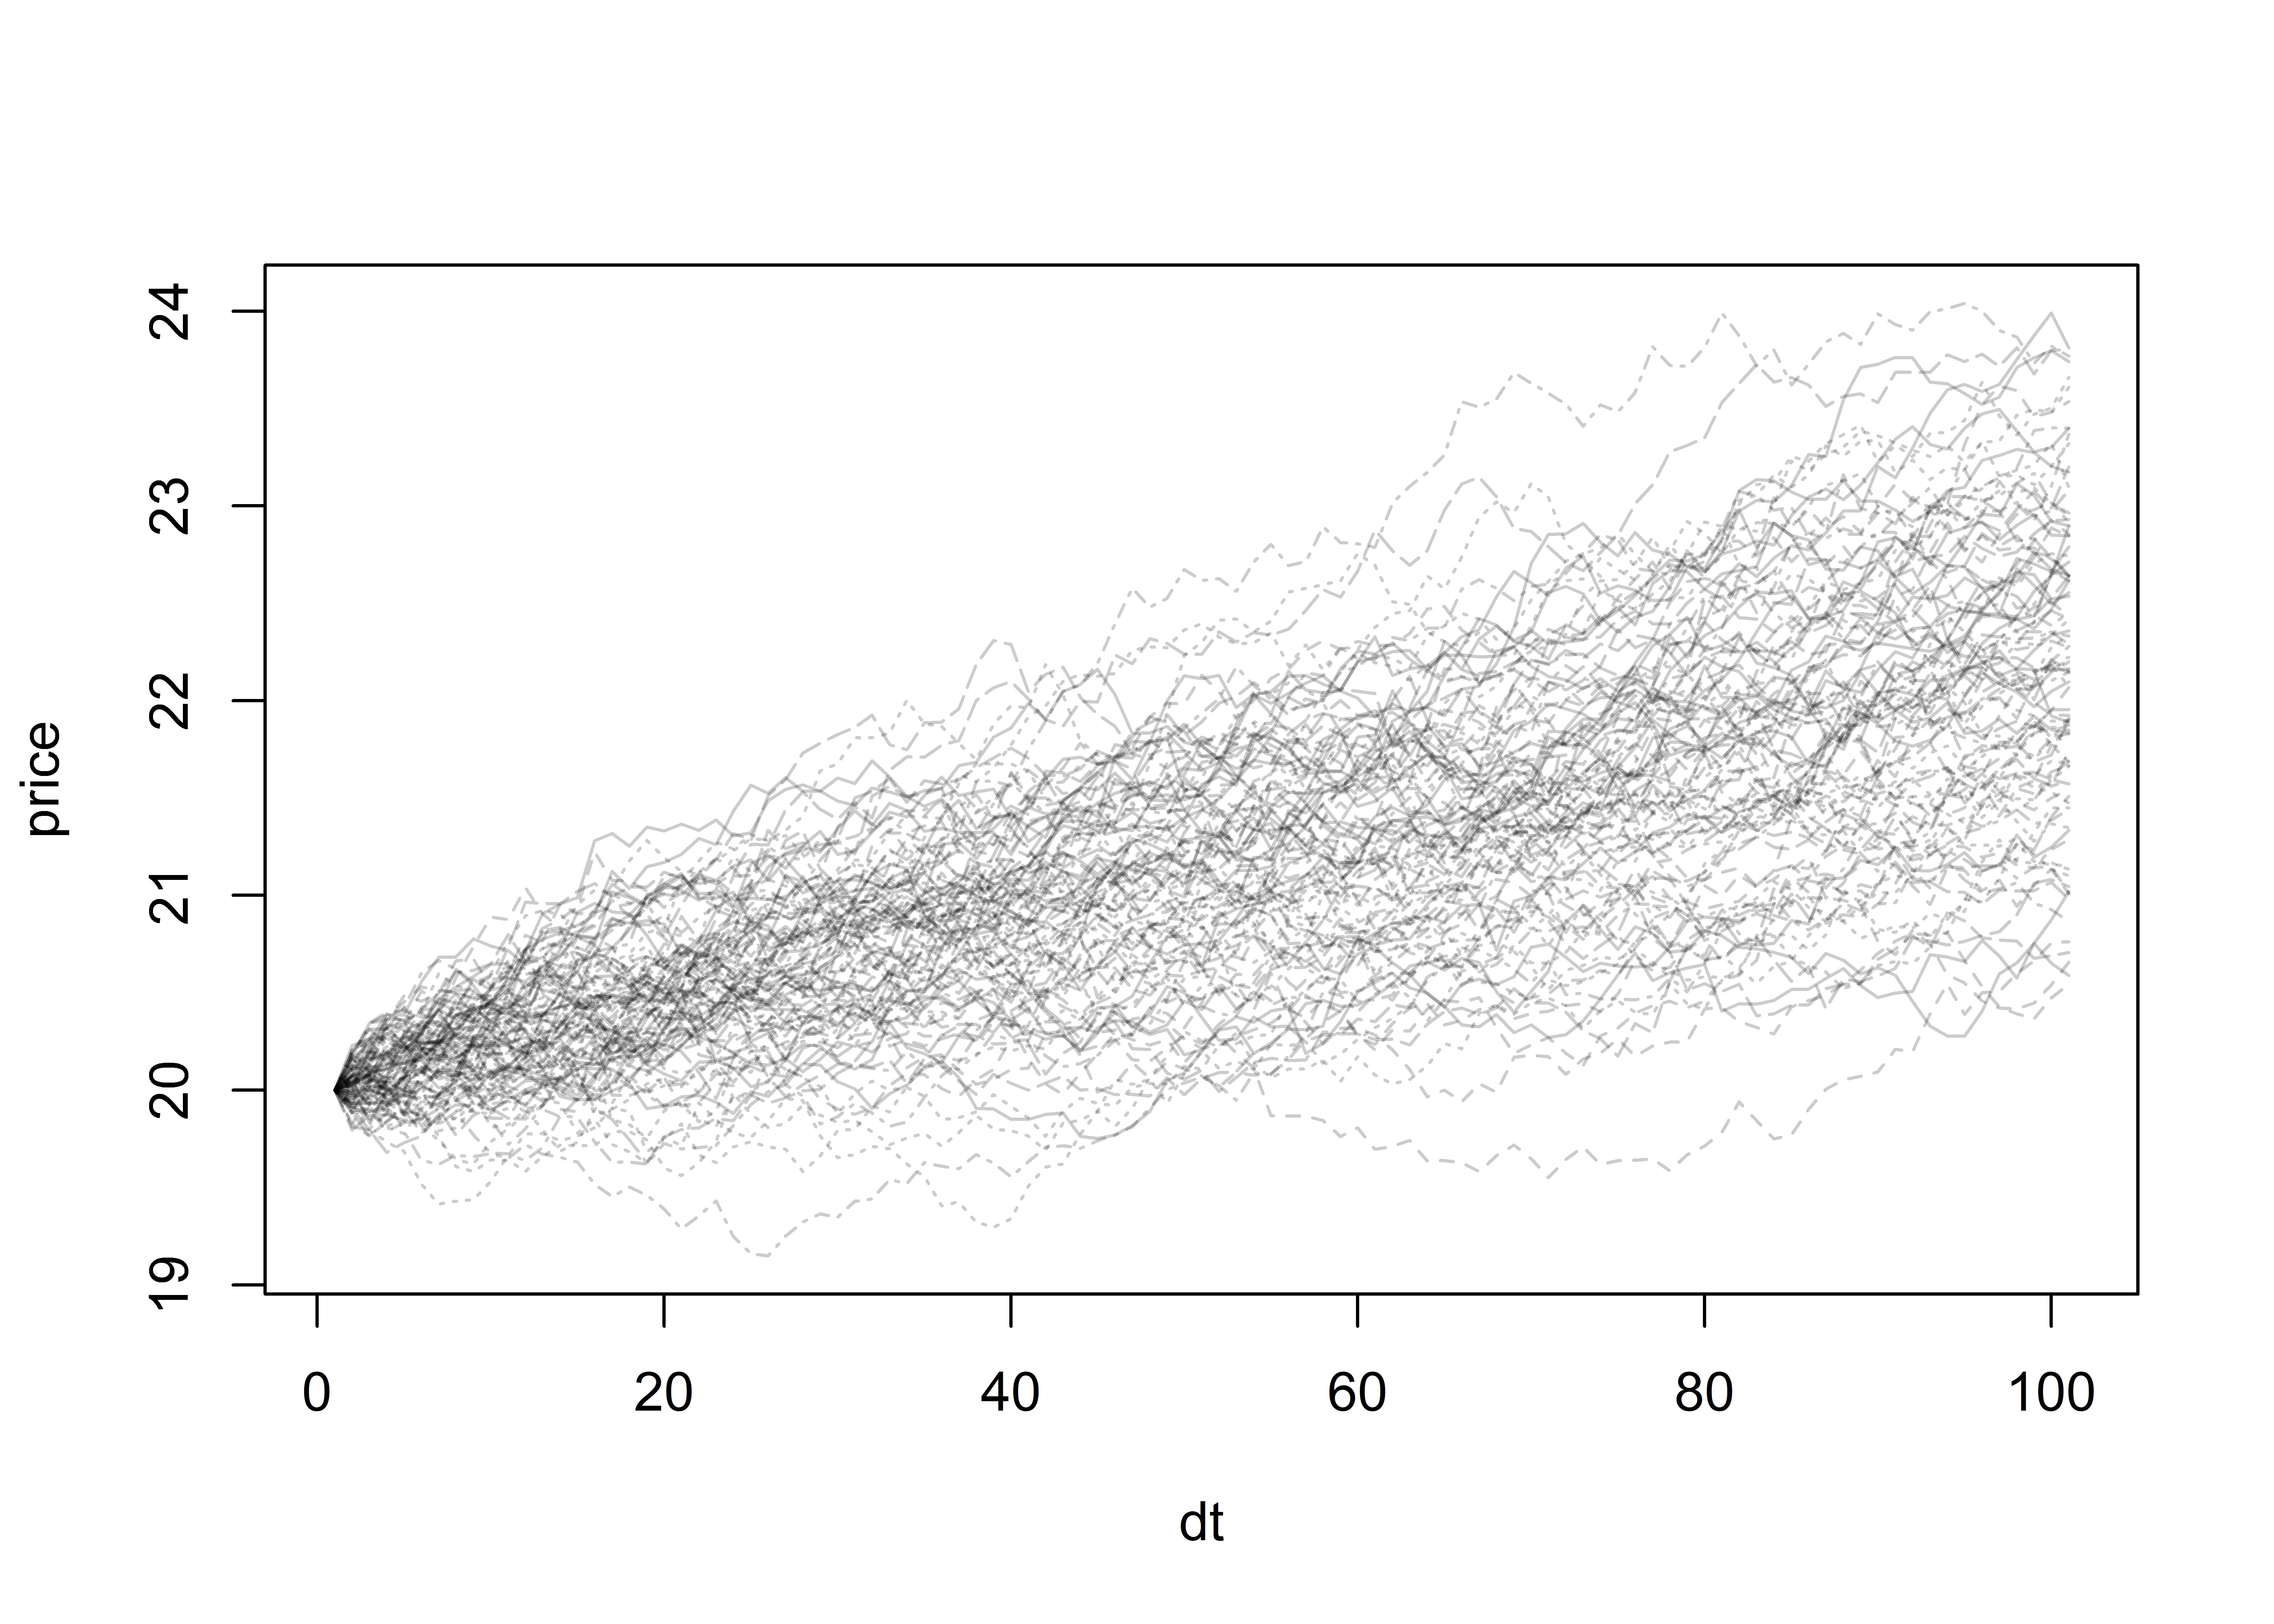
\includegraphics[scale = 0.5]{mc_trajectories.jpeg}
	\caption{Monte Carlo Price Trajectories} \label{img:mc_trajectories}
\end{figure}

From the result shown in Figure \ref{img:mc_trajectories}, we see an collectively upward movement for prices. This corresponds to our setup of a positive drift coefficient of $0.05$.

However, the above code is not computationally efficient. R is relatively slow in running for-loops, and we can speed up the process by using matrix method.

Recall Equation \ref{eq:BS_log_explicit}, where we have the explicit form of $\log(S_t)$. Using similar discretisation method, we can use standard normal random variable $Z$ to substitute $W_t$ to form a recursive equation, such that:

\begin{align*}
\log(S_i) = \log(S_{i-1}) + (\mu - \frac{\sigma^2}{2})\Delta t + \sigma Z_i \sqrt{\Delta t}
\end{align*}

Notice that assume $\Delta t$ is fixed, the part $\log(\Delta S)_i\coloneqq(\mu - \frac{\sigma^2}{2})\Delta t + \sigma Z_i \sqrt{\Delta t}$ is time independent. Therefore:

\begin{align}
\log(S_{i+k}) &= \log(S_{i-1}) + \sum_{j=i}^{k}{\left[(\mu - \frac{\sigma^2}{2})\Delta t + \sigma Z_i \sqrt{\Delta t}\right]} \\
&= \log(S_{i-1}) + \sum_{j=i}^{k}{\log(\Delta S_i)} \label{eq:mc_matrix}
\end{align}

For $i,k\in\mathbb{N}$ and $i+k\leq m$.

This allows us to reduce the two layers of for-loops into matrix operations.

\begin{Rminted}
mc.mat <- function() {
    Z <<- matrix(rnorm(n * m), ncol = n)
    logdS <<- (mu - sigma^2 / 2) * dt + sigma * Z * sqrt(dt)
    logS <<- log(S0) + apply(logdS, 2, cumsum)
    S <<- exp(logS)
    S <<- rbind(S0, S) # Add back the missing row of starting point S0
}
\end{Rminted}

Here, we first define \mintinline{R}|Z| to be a matrix that constains all standard normal random variables required for a total of $n\times m$ number of steps. Then we define \mintinline{R}|logdS| as the matrix of all increments. Based on Equation \ref{eq:mc_matrix}, by using $\log(S_0)$ as the starting point and use cumulative sum \mintinline{R}|cumsum| function to add increament $\log(\Delta S)$ along steps of each trajectory, we will obtain the movement of prices in time. By some further post process shown above, we will get the same result as using the for-loops.

To test the difference in computing speed between the two methods, we will test the average running time using the R package \mintinline{R}|microbenchmark|. The package's benchmarking test runs individual functions for 100 times and records the summary statistics of the running times, as shown below:

\begin{Rminted}
microbenchmark::microbenchmark(
    mc.for(),
    mc.mat()
)

    Unit: microseconds
    expr     min      lq      mean   median      uq     max neval
mc.for() 18327.2 19872.8 26257.504 25396.45 27853.6 60920.1   100
mc.mat()   831.8   964.9  1200.425  1039.30  1094.5  8045.3   100
\end{Rminted}

From the result we see that \mintinline{R}|mc.mat| is substantially faster than \mintinline{R}|mc.for|. We shoud thus prefer the former to obtain better estimation efficiency.

The matrix method can also be implemented via the form shown in Equation \ref{eq:mc_explicit} using cumulative product \mintinline{R}|cumprod| function. However, the running time for single multiplication is slightly longer than addition. One may decide to use either methods considering redability and efficiency.

The full look of the \mintinline{R}|mc.engine| is as such:

\begin{Rminted}
    mc.engine <- function(type, K, t, S0, r, q, sigma, n, steps) {

    dt <- t / steps

    # Generate n random samples from N(0,1)
    Z <- matrix(rnorm(n * steps), ncol = n)

    # Get logarithm of price change per step
    increment <- (r - q - sigma^2 / 2) * dt + sigma * sqrt(dt) * Z

    # Use vectorised MC method to compute logarithm of S(t) at each time step
    logS <- log(S0) + apply(increment, 2, cumsum)
    S <- exp(logS) # Obtain the simulated stock price by taking exponential
    S <- S * exp(-q * t) # Adjust the asset price for dividends
    S <- rbind(S0, S) # Add column of current price
    S
}
\end{Rminted}

Here, the drift coefficient is decomposed to (fixed) annual interest rate $r$ and (fixed) annual dividend yield rate $q$ according to Equation \ref{eq:mc_explicit_rq}. The number of time steps $m$ is directly named as \mintinline{R}|steps|.

Adapting this formulation, \mintinline{R}|rmcop| has a function named \mintinline{R}|mc.engine|, which takes the mentioned input arguments and returns a $(m+1)\times n$ matrix recording all generated trajectories. The rest of the functions described in the following subsections takes \mintinline{R}|mc.engine| as an internal component and use the returned matrix to perform further calculations of option payoff.

The Standard Error of estimation is then calculated according to Equation \ref{eq:mc_SE}, which is implemented directly using the below algorithm:

\begin{Rminted}
mc.SE <- function(C_i, C.mean, n) {
    s_c <- sqrt(sum(C_i - C.mean)^2 / (n - 1))
    SE <- s_c / sqrt(n)
    SE
}
\end{Rminted}

One should be aware that Monte Carlo option pricing for American options is beyond the scope of this report. In the pricing functions below, we will only consider the pricing of European options.

\subsection{vanilla.mc}

The pricing of Vanilla options is examplified in Equation \ref{eq:discount_vanilla_payoff}. To obtain the simulated $S_T$'s, one shall simply take the last row of the matrix output from the \mintinline{R}|mc.engine| and directly translate the formula to R code:

\begin{Rminted}
if (type == "call") {
    C <- exp(-r * t) * pmax(S[steps + 1, ] - K, 0)
} else if (type == "put") {
    C <- exp(-r * t) * pmax(K - S[steps + 1, ], 0)
}
\end{Rminted}

Notice that for a path-independent option such as an Vanilla option, we are only considering the option price at expiration. Thus, it is reasonable to take \mintinline{R}|step = 1| to reduce computational cost.

\subsection{asian.mc}

Exotic options such as Asian options and those included below are path-dependent. This implies capturing the price movements throughout time $t\in[0,T]$ is necessary.

Recall from Section \ref{sec:Literature Review}, an Asian option consider the average price. Thus, we shall first take the average of simulated price trajectories.

\begin{Rminted}
S.mean <- apply(S, 2, mean)
\end{Rminted}

\begin{Rminted}
if (is.avg_price) { # Compute payoff for average price Asian option
    if (type == "call") {
        C <- exp(-r * t) * pmax(S.mean - K, 0)
    } else if (type == "put") {
        C <- exp(-r * t) * pmax(K - S.mean, 0)
    }
} else { # Compute payoff for average strike Asian option
    if (type == "call") {
        C <- exp(-r * t) * pmax(S[steps + 1, ] - S.mean, 0)
    } else if (type == "put") {
        C <- exp(-r * t) * pmax(S.mean - S[steps + 1, ], 0)
    }
}
\end{Rminted}

\subsection{barrier.mc}

\subsection{binary.mc}

\subsection{lookback.mc}

\newpage